%%%%%%%%%%%%%%%%%%%%%%%%%%%%%%%%%%%%%%%%%%%%%%%%%%%%%%%%%%%%%%%%%%%%%%%%%
% This file is part of the LaTeX sources of the OMDoc 1.3 specification
% Copyright (c) 2016 Michael Kohlhase.
% Source at https://github.com/KWARC/OMDoc/tree/master/doc/spec
% This work is licensed by the Creative Commons Share-Alike license
% see http://creativecommons.org/licenses/by-sa/2.5/ for details
%%%%%%%%%%%%%%%%%%%%%%%%%%%%%%%%%%%%%%%%%%%%%%%%%%%%%%%%%%%%%%%%%%%%%%%%%

\begin{tchapter}[id=courseware]{Courseware and the Narrative/Content Distinction}

In this chapter we will look at another type of mathematical document:
{\indextoo{courseware}}; in this particular case a piece from an introductory
course ``{\indextoo{Fundamentals of Computer Science}}\twin{computer}{science}''
(Course 15-211 at {\indextoo{Carnegie Mellon University}}). The {\omdoc} documents
produced from such courseware can be used as input documents for {\activemath}
(see {\mysecref{activemath}}) and can be produced e.g. by {\cpoint} (see
{\mysecref{cpoint}}).

\begin{myfig}{15-211}{Three slides from 15-211}
  \fbox{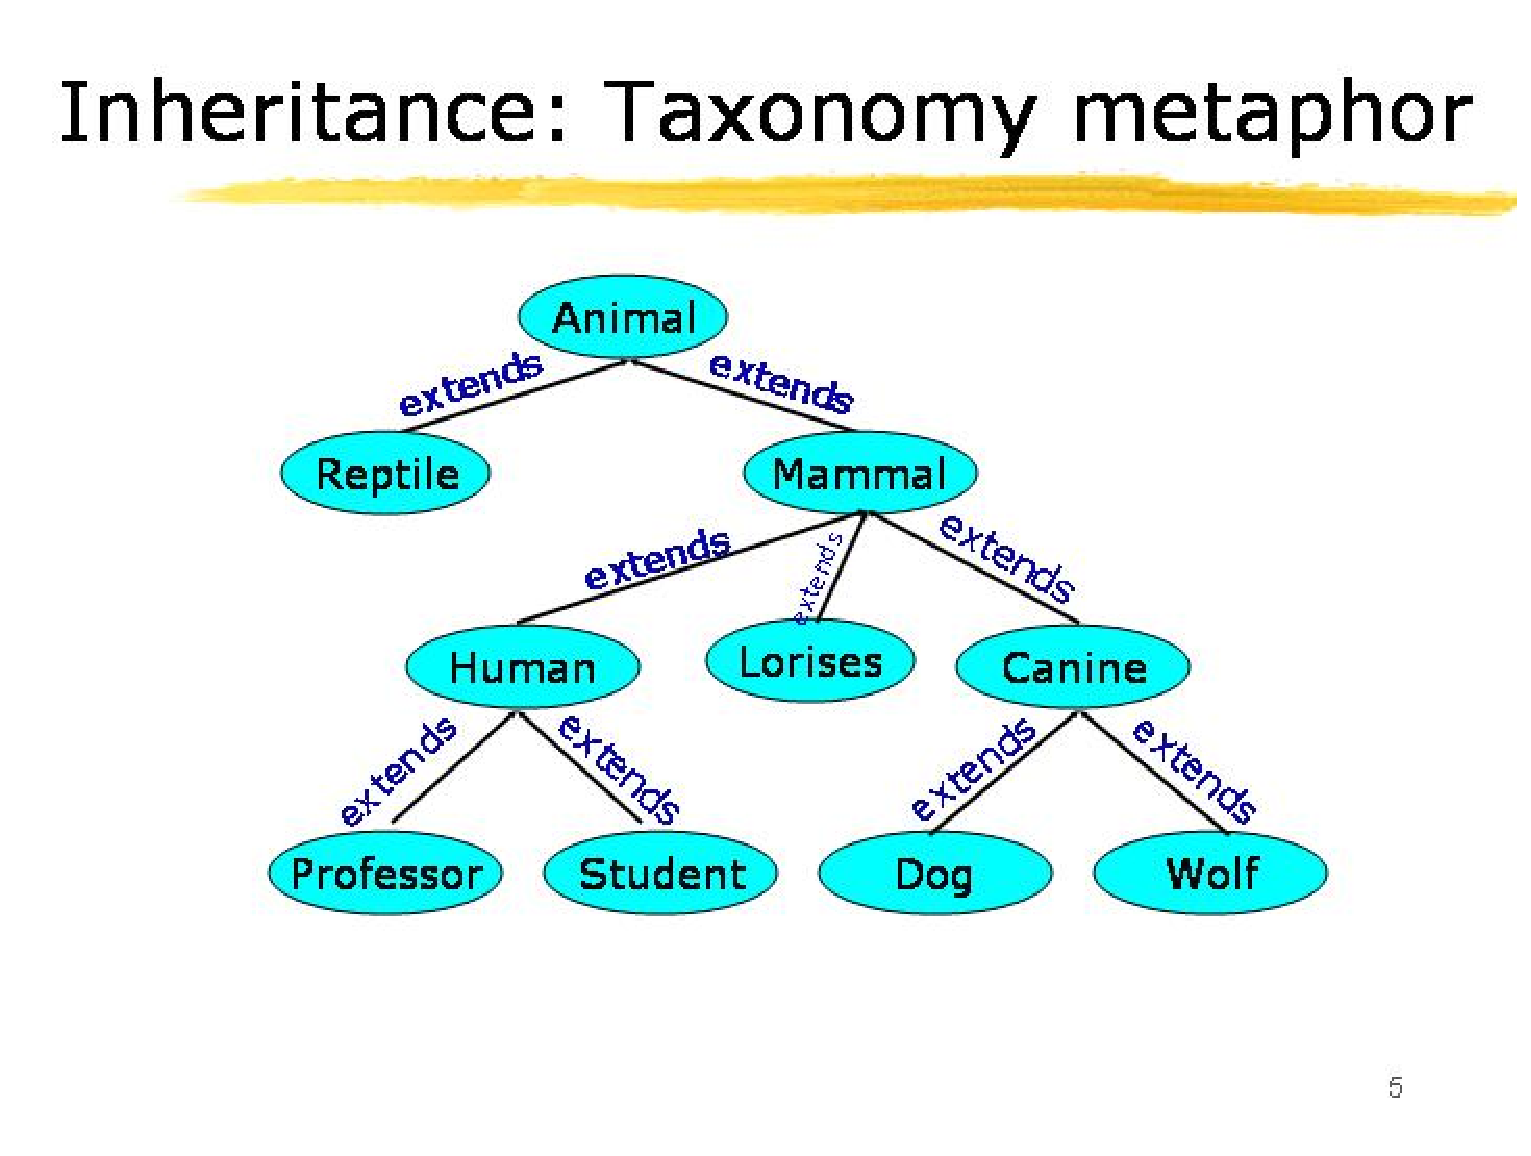
\includegraphics[width=5.2cm]{figures/slide-847}}\quad
  \fbox{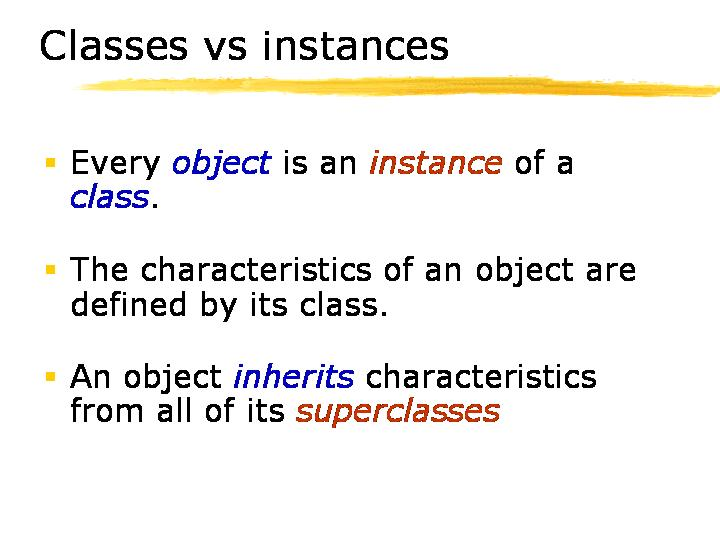
\includegraphics[width=5.2cm]{figures/slide-862}}\\[1ex]
  \fbox{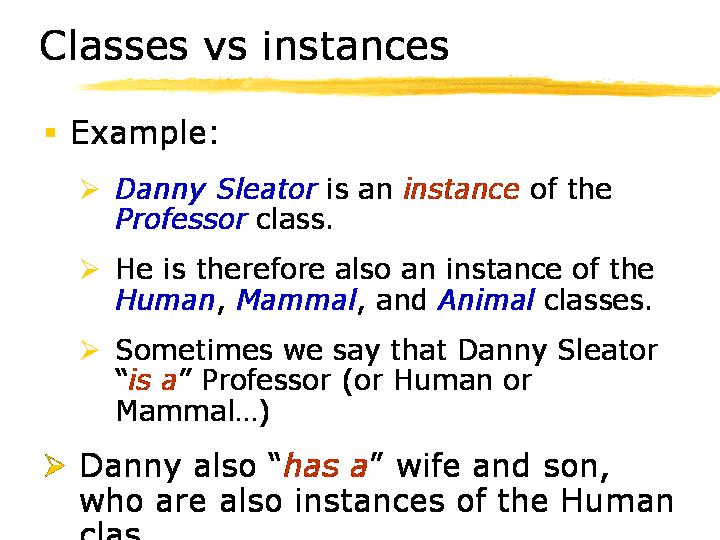
\includegraphics[width=5.2cm]{figures/slide-863}}\quad
  \fbox{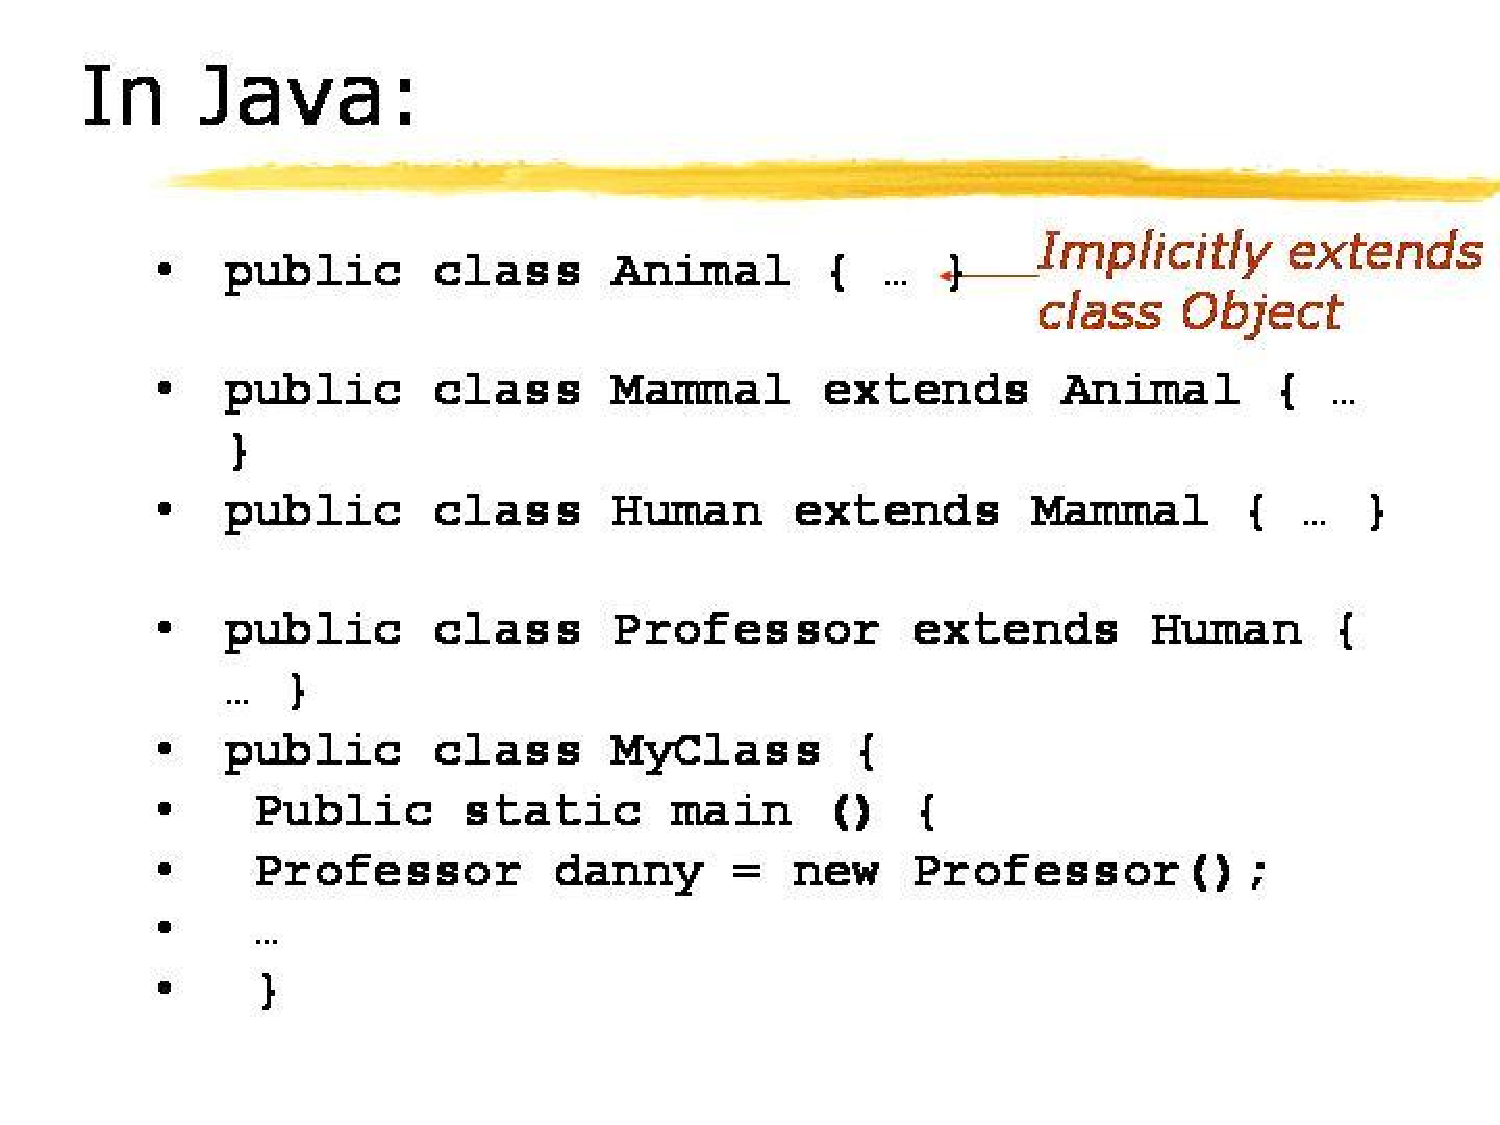
\includegraphics[width=5.2cm]{figures/slide-864}}
\end{myfig}

We have chosen a fragment that is relatively far from conventional mathematical
texts to present the possibility of semantic markup in {\omdoc} even under such
circumstances.  We will highlight the use of {\omdoc} theories\index{theory} for
such an application. Furthermore, we will take seriously the difference between
marking up the knowledge (implicitly) contained in the {\indextoo{slide}s} and the
{\indextoo{slide presentation}}\index{presentation!slides} as a structured
document. As a consequence, we will capture the slides in {\emph{two}} documents:

\begin{itemize}
\item a {\emph{knowledge-centered\twin{knowledge-centered}{document} document}}, which contains
  the knowledge conveyed in the course organized by its inherent logical structure
\item a {\emph{narrative-structured\twin{narrative-structured}{document} document}}
  references the knowledge items and adds rhetorical and didactic structure of a
  slide presentation.
\end{itemize}
This separation of concerns into two documents is good practice in marking up mathematical
texts: It allows to make explicit the structure inherent in the respective domain and at
the same time the structure of the presentation that is driven by didactic needs. We
call knowledge-structured documents {\twindef{content}{OMDoc}s} and narrative-structured
ones {\twindef{narrative}{OMDoc}s}.  The separation also simplifies management of academic
content\twin{content}{management}: The content {\omdoc} of course will usually be shared
between individual installments of the course, it will be added to,
{\indextoo{correct}ed}, {\indextoo{cross-reference}d}, and kept up to date by different
authors. It will eventually embody the institutional memory of an organization like a
university or a group of teachers.  The accompanying narrative {\omdoc}s will capture the
different didactic tastes and approaches by individual teachers and can be adapted for the
installments of the course. Since the narrative {\omdoc}s are relatively light-weight
structures (they are largely void of original content, which is referenced from the
content {\omdoc}) constructing or tailoring a course to the needs of the particular
audience becomes a simpler endeavor of choosing a path through a large repository of
marked up knowledge embodied in the content {\omdoc} rather than
re-authoring\footnote{Since much of the re-authoring is done by copy and paste in the
  current model, it propagates errors in the course materials rather than corrections.}
the content with a new slant.

Let us look at the four slides in {\myfigref{15-211}}. The first
{\indextoo{slide}} shows a graphic of a simple {\indextoo{taxonomy}} of
{\indextoo{animal}s}, the second one introduces first concepts from
{\twintoo{object-oriented}{programming}}, the
third one gives examples for these interpreting the class hierarchy introduced in
the first slide, finally the fourth slide gives code concrete snippets as examples
for the concepts introduced in the first three ones.

We will first discuss content {\omdoc} and then the narrative {\omdoc} in
{\mysecref{narrative-structured}}.

\begin{tsection}[id=knowledge-centered]{A Knowledge-Centered View}
  
  In this section, we will take a look at how we can make the knowledge that is contained
  in the slides in {\myfigref{15-211}} and its structure explicit so that a
  {\twintoo{knowledge}{management}} system like {\mbase} (see {\mysecref{mbase}}) or
  {\twintoo{knowledge}{presentation}} system like {\activemath} (see
  {\mysecref{activemath}}) can take advantage of it. We will restrict ourselves to
  knowledge that is explicitly represented in the slides in some form, even though the
  knowledge document would probably acquire more and more knowledge in the form of
  examples, graphics, variant definitions, and explanatory text as it is re-used in many
  courses.

The first slide introduces a theory, which we call {\snippet{animals-tax}}; see
{\mylstref{ann-tax}}.  It declares {\twintoo{primitive}{symbol}s} for all the
{\indextoo{concept}s}\footnote{The type information in the symbols is not strictly
  included in the slides, but may represent the fact that the instructor said that
  the ovals represent ``concepts''.}  (the ovals), and for all the links
introduced in the graphic it has {\element{axiom}} elements stating that the
parent node in the {\indextoo{tree}} extends the child node. The axiom uses the
symbol for {\twintoo{concept}{extension}} from a theory {\snippet{kr}} for
{\twintoo{knowledge}{representation}} which we import in the theory and which we
assume in the background materials for the course.

\begin{lstlisting}[label=lst:ann-tax,mathescape,
    caption={The {\omdoc} Representation for Slide 1 from {\myfigref{15-211}}},
    index={theory,axiom,symbol,CMP,FMP,OMA,OMOBJ,OMS,private,data}]
<theory xml:id="animals-tax">
  <imports xml:id="tax_imports_taxonomy" from="#taxonomies"/>
  <imports xml:id="tax_imports_kr" from="#kr"/>
  <symbol name="human">
    <type system="stlc"><OMOBJ><OMS cd="kr" name="concept"/></OMOBJ></type>
  </symbol>
  <symbol name="mammal">
    <type system="stlc"><OMOBJ><OMS cd="kr" name="concept"/></OMOBJ></type>
  </symbol>
  $\ldots$
  <axiom xml:id="mammal-ext-human">
    <CMP><xhtml:p>Humans are Animals.</xhtml:p></CMP>
    <FMP>
      <OMOBJ>
        <OMA><OMS cd="kr" name="extends"/>
          <OMS cd="animal-taxonomy" name="mammal"/>
          <OMS cd="animal-taxonomy" name="human"/>
        </OMA>
      </OMOBJ>
    </FMP>
  </axiom>
  $\ldots$
</theory>

<private xml:id="tax-image" for="#animals-tax" reformulates="#animals-tax">
  <data format="image/jpeg" href="animals-taxonomy.jpg"/>
  <data format="application/postscript" href="animals-taxonomy.ps"/>
</private>
\end{lstlisting}
The {\element{private}} element contains the reference to the image in various
formats. Its {\attribute{reformulates}{private}} attribute hints that the image
contained in this element can be used to illustrate the theory above (in fact, it
will be the only thing used from this theory in the narrative {\omdoc} in
{\mylstref{ann-narrative}}.)

The second slide introduces some basic concepts in object oriented programming.  These
give rise to the five {\twintoo{primitive}{symbol}s} of the theory. Note that this theory
is basic, it does not import any other. The three text blocks are marked up as axioms,
using the attribute {\attribute{for}{axiom}} to specify the symbols involved in these
axioms. The value of the {\attribute{for}{axiom}} attribute is a whitespace-separated list
of {\twintoo{URI}{reference}s} to {\element{symbol}} elements.

\begin{lstlisting}[label=lst:ann-oo,
    caption={The {\omdoc} Representation for Slide 2 from {\myfigref{15-211}}},
    index={theory,axiom,symbol,CMP,FMP,OMA,OMOBJ,OMS}]
<theory xml:id="cvi">
  <symbol name="object" xml:id="cvi.object"/>
  <symbol name="instance" xml:id="cvi.instance"/>
  <symbol name="class" xml:id="cvi.class"/>
  <symbol name="inherits" xml:id="cvi.inherits"/>
  <symbol name="superclass" xml:id="cvi.superclass"/>

  <axiom xml:id="ax1" for="object instance class">
    <CMP>
      <xhtml:p>
        Every <xhtml:span style="font-style:italic;color:blue">object</xhtml:span>
        is an <xhtml:span style="font-style:italic;color:red">instance</xhtml:span> 
        of a <xhtml:span style="font-style:italic;color:blue">class</xhtml:span>.
     </xhtml:p>
    </CMP>
  </axiom>

  <axiom xml:id="ax2" for="class">
    <CMP><xhtml:p>The characteristics of an object are defined by its class.</xhtml:p></CMP>
  </axiom>

  <axiom xml:id="ax3" for="inherits superclass">
    <CMP><xhtml:p>An object <xhtml:span style="font-style:italic;color:blue">inherits</xhtml:span>
      characteristics from all of its 
      <xhtml:span style="font-style:italic;color:red">superclasses</xhtml:span>.</xhtml:p></CMP>
   </axiom>
</theory>
\end{lstlisting}

For the third slide it is not entirely obvious which of the {\omdoc} elements we want to
use for markup. The intention of the slide is obviously to give some {\indextoo{example}s}
for the concepts introduced in the second slide in terms of the taxonomy presented in the
first slide in {\myfigref{15-211}}. However, the {\omdoc} {\element{example}} element
seems to be too specific to directly capture the contents (see
p.~\pageref{eldef:example}). What is immediately obvious is that the slide introduces some
new knowledge and symbols, so we have to have a separate theory for this slide. The first
item in the list headed by the word Example is a piece of new knowledge, it is therefore
not an example at all, but an axiom\footnote{We could say that the function of being an
  example has moved up from mathematical statements to mathematical theories; we will not
  pursue this here.}. The second item in the list is a statement that can be deduced from
the knowledge we already have at our disposal from theories {\snippet{animals-tax}}
and {\snippet{cvi}}.  Therefore, the new theory {\snippet{cvi-examples}} in
{\mylstref{ann-cvi-ex}} imports these two. Furthermore, it introduces the new symbol
{\snippet{danny}} for ``Danny Sleator'' which is clarified in the {\element{axiom}}
element with {\snippet{xml:id="ax1"}}. Finally, the third item in the list does not have
the function of an example either, it introduces a new concept, the ``is a''
relation{\index{isa@``is a'' relation}}\index{relation!``is a''}\footnote{Actually, this
  text block introduces a new concept ``by reference to examples'', which is not a formal
  definition at all. We will neglect this for the moment.}.  So we arrive at the theory in
{\mylstref{ann-cvi-ex}}.  Note that this markup treats the last text block on the third
slide without semantic function in the theory -- it points out that there are other
relations among humans -- and leaves it for the narrative-structured {\omdoc} in
{\mysecref{narrative-structured}}\footnote{Of course this design decision is debatable,
  and depends on the intuitions of the author.  We have mainly treated the text this way
  to show the possibilities of semantic markup}.

\begin{lstlisting}[label=lst:ann-cvi-ex,
    caption={The {\omdoc} Representation for Slide 3 from {\myfigref{15-211}}},
    index={theory,imports,axiom,symbol,assertion,definition,CMP}]
<theory xml:id="cvi-examples">
  <imports from="#animals-tax"/><imports from="#cvi"/>

  <symbol name="danny" xml:id="cvi-examples.danny">
    <metadata><dc:description>Danny Sleator</dc:description></metadata>
  </symbol>

  <axiom xml:id="danny-professor" for="class instance danny">
    <CMP>
      <xhtml:p>
        <xhtml:span style="font-style:italic;color:blue">Danny Sleator</xhtml:span>
       is an <xhtml:span style="font-style:italic;color:red">instance</xhtml:span> 
       of the <xhtml:span style="font-style:italic;color:blue">Professor</xhtml:span> 
       class.
      </xhtml:p>
    </CMP>
  </axiom>

  <assertion xml:id="dannys-classes" type="theorem">
    <CMP>
      <xhtml:p>
        He is therefore also an instance of the 
        <xhtml:span style="font-style:italic;color:blue">Human</xhtml:span>, 
        <xhtml:span style="font-style:italic;color:blue">Mammal</xhtml:span>, 
        <xhtml:span style="font-style:italic;color:blue">Animal</xhtml:span> classes.
      </xhtml:p>
    </CMP>
  </assertion>

  <symbol name="is_a" scope="global">
    <metadata><dc:subject>'is a' relation</dc:subject></metadata>
  </symbol>

  <definition xml:id="is_a-def" for="is_a" type="informal">
     <CMP>
        <xhtml:p>Sometimes we say that Danny Sleator 
         &#x201C;<xhtml:span style="font-style:italic;color:red">is a</xhtml:span>&#x201D; 
         Professor (or Human or Mammal&#x2026;)
       </xhtml:p>
     </CMP>
  </definition>
</theory>
\end{lstlisting}

An alternative, more semantic way to mark up the {\element{assertion}} element in the
theory above would be to split it into multiple {\element{assertion}} and
{\element{example}} elements, as in {\mylstref{var-cvi-ex}}, where we have also added
formal content. We have split the {\indextoo{assertion}} {\snippet{dannys-classes}} into
three --- we have only shown one of them in {\mylstref{var-cvi-ex}} --- separate
assertions about class instances, and used them to justify the explicit examples. These
are given as {\omdoc} {\element{example}} elements. The {\attribute{for}{example}}
attribute of an {\element{example}} element points to the concepts that are exemplified
here (in this case the symbols for the {\indextoo{concept}s} ``instance'', ``class'' from
the theory {\snippet{cvi}} and the concept ``mammal'' from the animal taxonomy). The
{\attribute{type}{example}} specifies that this is not a {\indextoo{counter-example}}, and
the {\attribute{assertion}{example}} points to the justifying assertion. In this
particular case, the reasoning behind the example is pretty straightforward (therefore it
has been omitted in the slides), but we will make it explicit to show the mechanisms
involved. The {\element{assertion}} element just re-states the assertion implicit in the
example, we refrain from giving the formal statement in an {\element{FMP}} child here to
save space. The {\attribute{just-by}{assertion}} can be used to point to set of proofs for
this assertion, in this case only the one given in {\mylstref{var-cvi-ex}}. We use the
{\omdoc} {\element{proof}} element to mark up this proof.  It contains a series of
{\element{derive}} proof steps. In our case, the argument is very simple, we can see that
Danny Sleator is an instance of the human class, using the knowledge that
\begin{enumerate}
\item Danny is a professor (from the axiom in the {\snippet{cvi-examples}} theory)
\item An object inherits all the characteristics from its superclasses (from the
  axiom {\snippet{ax3}} in the {\snippet{cvi}} theory)
\item The human class is a superclass of the professor class (from the axiom
  {\snippet{human-extends-professor}} in the {\snippet{animal-taxonomy}} theory).
\end{enumerate}
The use of this knowledge in the proof step is made explicit by the
{\element{premise}} children of the {\element{derive}} element.

The information in the proof could for instance be used to generate very detailed
explanations for students who need help understanding the content of the original
slides in {\myfigref{15-211}}.


\begin{lstlisting}[label=lst:var-cvi-ex,mathescape,
    caption={An Alternative Representation Using {\element{example}} Elements},
    index={example,proof,assertion,derive,premise}]
$\ldots$
<example xml:id="danny-mammal" type="for" assertion="#dannys-mammal-thm"
         for="#cvi.instance #cvi.class #animal-taxonomy.mammal">
  <CMP><xhtml:p>Danny Sleator is an instance of the 
    <xhtml:span style="font-style:italic;color:blue">Mammal</xhtml:span> class. 
  <xhtml:p></CMP>
  <OMOBJ><OMS cd="cvi-examples" name="danny"/></OMOBJ>
</example>

<assertion xml:id="dannys-mammal-thm" type="theorem" proofs="#danny-mammal-pf">
  <CMP><xhtml:p>Danny Sleator is an instance of the Human class.</xhtml:p></CMP>
</assertion>

<proof xml:id="danny-human-pf" for="#dannys-mammal-thm">
  <derive xml:id="d1">
    <CMP><xhtml:p>Danny Sleator is an instance of the human class.</xhtml:p></CMP>
    <method>
      <premise xref="#danny-professor"/>
      <premise xref="#cvi.ax3"/>
      <premise xref="#animal-tax.human-extends-professor"/>
    </method>
  </derive>
  <derive xml:id="concl">
    <CMP><xhtml:p>Therefore he is an instance of the human class.</xhtml:p></CMP>
    <method>
      <premise xref="#d1"/>
      <premise xref="#cvi.ax3"/>
      <premise xref="#animal-tax.mammal-extends-human"/>
    </method>
  </derive>
</proof>
$\ldots$
\end{lstlisting}

The last slide contains a set of {\indextoo{Java}} {\twintoo{code}{fragment}s} that are
related to the material before.  We have marked them up in the {\element{code}} elements
in {\mylstref{cvi-code}}. The actual code is encapsulated in a {\element{data}} element,
whose {\attribute{format}{data}} specifies the format the data is in. The program text is
encapsulated in a {\indextoo{CDATA}} section to suspend the {\xml} {\indextoo{parser}}
(there might be characters like {\snippet{<}} or {\snippet{\&}} in there which offend it).
The {\element{code}} elements allow to document the {\indextoo{input}},
{\indextoo{output}}, and {\indextoo{side-effect}s} in {\element{input}},
{\element{output}}, {\element{effect}} elements as children of the {\element{code}}
elements. Since the code fragments in question do not have input or output, we have only
described the side-effect (class declaration and class extension). As the code elements do
not introduce any new symbols, definitions or axioms, we do not have to place them in a
theory. The second {\element{code}} element also carries a {\attribute{requires}{code}}
attribute, which specifies that to execute this code snippet, we need the previous one. An
application can use this information to make sure that one is loaded before executing this
code fragment.

\begin{lstlisting}[label=lst:cvi-code,mathescape,
    caption={{\omdoc} Representation of Program Code},
    index={code,data,CDATA,effect}]
<code xml:id="cvic-code1">
  <data format="Java"><![CDATA[public class Animal {$\ldots$ }]]></data>
  <effect><CMP>class declaration</CMP></effect>
</code>

<code xml:id="cvic-code2" requires="cvic-code1" >
  <data format="Java"><![CDATA[public class Mammal extends Animal {$\ldots$}]]></data>
  <effect><CMP>class extension</CMP></effect>
</code>
$\ldots$
\end{lstlisting}
\end{tsection}

\begin{tsection}[id=narrative-structured]{A Narrative-Structured View}

In this section we present an {\omdoc} document that captures the structure of the
slide show as a document. It references the knowledge items from the theories
presented in the last section and adds rhetorical and didactic structure of a
slide presentation.

The individual slides are represented as {\element{omgroup}} elements with
{\attribute{type}{omgroup}} {\attval{slide}{type}{omgroup}}.

The representation of the first slide in {\myfigref{15-211}} is rather straightforward: we
use the {\element[ns-elt=dc]{title}} element in {\element{metadata}} to represent the slide title.
Its {\attribute[ns-elt=dc]{class}{title}} attribute references a {\css} {\snippet{class}}
definition\twin{CSS}{class definition} in a style file. To represent the image with the
{\indextoo{taxonomy}} tree we use an {\element{omtext}} element with an {\element{omlet}}
element.

The second slide marks up the list structure of the slide with the {\element{omgroup}}
element (the value {\attval{itemize}{type}{omgroup}} identifies it as an itemizes
list). The items in the list are given by {\omdoc} references (see Section~\ref{flattening}) to
the axioms in the knowledge-structured document (see {\mylstref{ann-oo}}). The effect of
this markup is shared between the document: the content of the axioms are copied over from
the knowledge-structured document, when the narrative-structured is presented to the
user. However, the {\omdoc} references cascades its {\attribute{style}{ref}} attribute
(and the {\attribute{class}{ref}} attribute, if present) with the {\attribute{style}{ref}}
and {\attribute{class}{ref}} attributes of the target element, essentially adding style
directives during the copying process (see Section~\ref{tref-css-cascading} for details). In our
example, this adds positioning information and specifies a particular image for the list
bullet type.

\begin{lstlisting}[label=lst:ann-narrative,mathescape,
    caption={The Narrative {\omdoc}  for {\myfigref{15-211}}},
    index={omgroup,omtext,CMP,metadata,dc:title,ref}]
$\ldots$
<omgroup xml:id="slide-847" type="slide">
  <metadata>
    <dc:title class="15-211-title">Inheritance: Taxonomy metaphor</dc:title>
  </metadata>
  
  <omtext xml:id="the-tax">
    <CMP><xhtml:p>
      <omlet data="#tax-image" style="width:540;height:366" 
             action="display" show="embed"/></xhtml:p>
    </CMP>
  </omtext>
</omgroup>

<omgroup xml:id="slide-848" type="slide">
  <metadata><dc:title class="15-211-title">Classes vs. instances</dc:title></metadata>
  <omgroup type="itemize" style="list-style-type:url(square.gif)">
    <axiom style="position:30% 10%" xml:id="obj" xref="slide1_content.omdoc#ax1"/>
    <axiom style="position:55% 10%" xml:id="class" xref="slide1_content.omdoc#ax2"/>
    <axiom style="position:80% 10%" xml:id="inh" xref="slide1_content.omdoc#ax3"/>
  </omgroup>
</omgroup>

<omgroup xml:id="slide-849" type="slide">
  <metadata><dc:title class="15-211-title">Classes vs. instances</dc:title></metadata>
  <omgroup type="itemize" style="list-style-type:url(square.gif)">
    <omtext style="position:30% 10%" xml:id="ex"><CMP><xhtml:p>Example:</xhtml:p></CMP></omtext>
    <omgroup type="itemize" style="list-style-type:url(triangle.gif)">
      <axiom style="position:400% 15%" 
           xml:id="danny" xref="slide1_content.omdoc#danny-professor"/>
      <axiom style="position:55% 15%" 
           xml:id="inst" xref="slide1_content.omdoc#dannys-classes"/>
      <axiom style="position:70% 15%" xml:id="is_a" xref="slide1_content.omdoc#is_a-def"/>
    </omgroup>
    <omtext style="position:83% 10%" xml:id="has_a">
      <CMP>
        <xhtml:p>Danny also &#x201C;<xhtml:span style="font-style:italic;color:red">has
        a</xhtml:span>&#x201D; wife and son, who are also instances of the Human class
      </xhtml:p></CMP>
    </omtext>
  </omgroup>
</omgroup>

<omgroup xml:id="slide-850" type="slide">
  <metadata><dc:title class="15-211-title">In Java</dc:title></metadata>
  <omgroup type="itemize">
    <omtext xml:id="slide-850.t1" style="position:80% 10%;color:red">
      <CMP><xhtml:p>Implicitly extends class object</xhtml:p></CMP>
    </omtext>
    <omtext xml:id="slide-850.t2">
      <CMP><xhtml:p><omlet data="#cvic-code1" action="display" show="embed"/></xhtml:p></CMP>
    </omtext>
    <omtext xml:id="slide-850.t3">
      <CMP><xhtml:p><omlet data="#cvic-code2" action="display" show="embed"/></xhtml:p></CMP>  
    </omtext>
  </omgroup>
</omgroup>
$\ldots$
\end{lstlisting}
\end{tsection}

\begin{tsection}[id=choreographing]{Choreographing  Narrative and Content OMDoc}

The interplay between the narrative and content {\omdoc} above was relatively
simple. The content {\omdoc} contained three theories that were linearized
according to the dependency relation. This is often sufficient, but more complex
{\twintoo{rhetoric/didactic}{figure}s}\twin{didactic}{figure} are also
possible. For instance, when we introduce a new concept, we often first introduce
a naive reduced approximation $\cal N$ of the real theory $\cal F$, only to show an example
$\cal E_N$ of where this is insufficient. Then we propose a first (straw-man)
solution $\cal S$, and show an example $\cal E_S$ of why this does not work. Based
on the information we gleaned from this failed attempt, we build the eventual
version $\cal F$ of the concept or theory and demonstrate that this works on $\cal
E_F$.

Let us visualize the narrative- and content structure in {\myfigref{straw-man}}. The
structure with the solid lines and boxes at the bottom of the diagram represents the
content structure, where the boxes $\cal N$, $\cal E_N$, $\cal S$, $\cal E_S$,
$\cal F$, and $\cal E_F$ signify theories for the content of the respective
concepts and examples, much in the way we had them in
{\mysecref{knowledge-centered}}. The arrows represent the
{\twintoo{theory}{inheritance}} structure, e.g. Theory $\cal F$ imports theory
$\cal N$.

\begin{myfig}{straw-man}{An Introduction of a Concept via a Straw-Man Theory}
  %%%%%%%%%%%%%%%%%%%%%%%%%%%%%%%%%%%%%%%%%%%%%%%%%%%%%%%%%%%%%%%%%%%%%%%%%
% This file is part of the LaTeX sources of the OMDoc 1.3 specification
% Copyright (c) 2016 Michael Kohlhase.
% Source at https://github.com/KWARC/OMDoc/tree/master/doc/spec
% This work is licensed by the Creative Commons Share-Alike license
% see http://creativecommons.org/licenses/by-sa/2.5/ for details
%%%%%%%%%%%%%%%%%%%%%%%%%%%%%%%%%%%%%%%%%%%%%%%%%%%%%%%%%%%%%%%%%%%%%%%%%

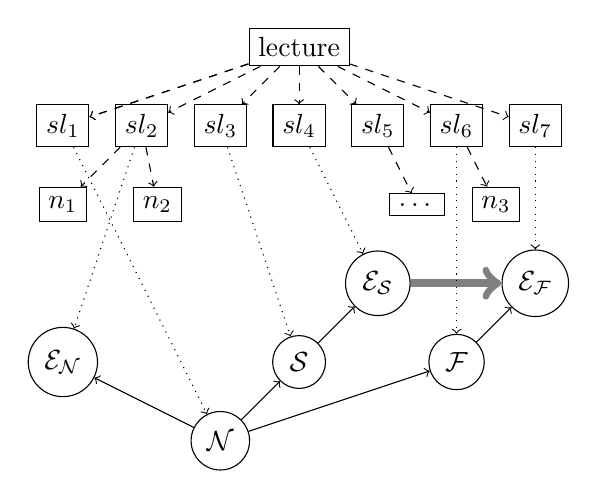
\begin{tikzpicture}
  \begin{scope}[shape=circle]
    \tikzstyle{every node}=[draw]
    \node (N)  at (2,0.5) {$\cal N$};
    \node (EN) at (0,1.5) {$\cal E_N$};
    \node (F)  at (5,1.5) {$\cal F$};
    \node (S)  at (3,1.5) {$\cal S$};
    \node (EF) at (6,2.5) {$\cal E_F$};
    \node (ES) at (4,2.5) {$\cal E_S$};
  \end{scope}
  \draw[->] (N) -- (EN);
  \draw[->] (N) -- (F);
  \draw[->] (N) -- (S);
  \draw[->] (S) -- (ES);
  \draw[->] (F) -- (EF);
  \draw[->,gray,line width=3pt] (ES) -- (EF);
  \begin{scope}
    \tikzstyle{every node}=[draw]
  \node (top) at (3,5.5) {lecture};
  \node (sl1) at (0,4.5) {$sl_1$};
  \node (sl2) at (1,4.5) {$sl_2$};
  \node (sl3) at (2,4.5) {$sl_3$};
  \node (sl4) at (3,4.5) {$sl_4$};
  \node (an) at (4,4.5) {$sl_5$};
  \node (sl5) at (5,4.5) {$sl_6$};
  \node (sl6) at (6,4.5) {$sl_7$};
  \node (n1) at (0,3.5) {$n_1$};
  \node (n2) at (1.2,3.5) {$n_2$};
  \node (n5) at (4.5,3.5){\ldots};
  \node (n6) at (5.5,3.5) {$n_3$};
\end{scope}
  \draw[->,dashed] (top) -- (sl1);
  \draw[->,dashed] (top) -- (sl1);
  \draw[->,dashed] (top) -- (sl2);
  \draw[->,dashed] (top) -- (sl3);
  \draw[->,dashed] (top) -- (sl4);
  \draw[->,dashed] (top) -- (an);
  \draw[->,dashed] (top) -- (sl5);
  \draw[->,dashed] (top) -- (sl6);
  \draw[->,dashed] (sl2) -- (n1);
  \draw[->,dashed] (sl2) -- (n2);
  \draw[->,dashed] (an) -- (n5);
  \draw[->,dashed] (sl5) -- (n6);

  \draw[->,dotted] (sl1) -- (N);
  \draw[->,dotted] (sl2) -- (EN);
  \draw[->,dotted] (sl3) -- (S);
  \draw[->,dotted] (sl4) -- (ES);
  \draw[->,dotted] (sl5) -- (F);
  \draw[->,dotted] (sl6) -- (EF);
\end{tikzpicture}

%%% Local Variables: 
%%% mode: latex
%%% TeX-master: "omdoc"
%%% End: 

% LocalWords:  EF sl

\end{myfig}

The top part of the diagram with the dashed lines stands for the narrative structure,
where the arrows mark up the document structure. For instance, the slides {sl$_i$} are
grouped into a lecture. The dashed lines between the two documents visualize {\omdoc}
references with pointers into the content structure. In the example in
{\myfigref{straw-man}}, the second slide of ``lecture'' presents the first example: the
text fragment {n$_1$} links the content $\cal E_N$, which is referenced from the content
structure, to slide 1. The fragment {n$_2$} might say something like ``this did not work
in the current situation, so we have to extend the conceptualization\ldots''.

Just as for content-based systems on the formula level, there are now MKM systems that
generate presentation markup from content markup, based on general presentation
principles, also on this level. For instance, the {\sc{ActiveMath}}
system~\cite{MelBue:krma03} generates a simple narrative structure (the
presentation; called a personalized book) from the underlying content structure (given in
{\omdoc}) and a user model.
\end{tsection}

\begin{tsection}[id=courseware-summary]{Summary}
As we have seen, the narrative and content fulfill different, but legitimate
content markup needs, that can coincide (as in the main example in this chapter),
but need not (as in the example in the last section). In the simple case, where
the dependency and narrative structure largely coincide, systems like the
{\activemath} system described in {\mysecref{activemath}} can generate narrative
{\omdoc}s from content {\omdoc}s automatically. To generate more complex
{\twintoo{rhetoric/didactic}{figure}s}\twin{didactic}{figure}, we would have to
have more explicit markup for relations like ``can act as a straw-man for''.
Providing standardized markup for such relations is beyond the scope of the
{\omdoc} format, but could easily be expressed as metadata, or as external, e.g.
{\rdf}-based relations.
\end{tsection}
\end{tchapter}


%%% Local Variables: 
%%% mode: latex
%%% TeX-master: "omdoc"
%%% End: 

% LocalWords:  ann kr lst stlc cd ext href jpg ps oo cvi danny pf uri url
% LocalWords:  superclasses Sleator isa dannys def var xref concl EN dc ns elt
% LocalWords:  pto cvic omlet ref otheromgrouptype obj inh inst activemath gif
% LocalWords:  cpoint omcds mowgli EF ES linecolor linewidth sl RDF clas xunit
% LocalWords:  mathescape Courseware courseware mbase CMP FMP OMA OMOBJ thm
% LocalWords:  metadata CDATA omgroup omtext omdoc ActiveMath  ActiveMath
% LocalWords:  ActiveMath MelBue krma03
